%%%%%%%% ICML 2021 EXAMPLE LATEX SUBMISSION FILE %%%%%%%%%%%%%%%%%

\documentclass{article}

% Recommended, but optional, packages for figures and better typesetting:
\usepackage{microtype}
\usepackage{graphicx}
\usepackage{subfigure}
\usepackage{booktabs} % for professional tables

% hyperref makes hyperlinks in the resulting PDF.
% If your build breaks (sometimes temporarily if a hyperlink spans a page)
% please comment out the following usepackage line and replace
% \usepackage{icml2021} with \usepackage[nohyperref]{icml2021} above.
\usepackage{hyperref}

% Attempt to make hyperref and algorithmic work together better:
\newcommand{\theHalgorithm}{\arabic{algorithm}}

% Use the following line for the initial blind version submitted for review:
% \usepackage{icml2021}

% If accepted, instead use the following line for the camera-ready submission:
\usepackage[accepted]{icml2021}

% The \icmltitle you define below is probably too long as a header.
% Therefore, a short form for the running title is supplied here:
\icmltitlerunning{Is $\epsilon=12.2$ private?}

\begin{document}

\twocolumn[
\icmltitle{Disclosure avoidance in redistricting data: is $\epsilon=12.2$ private?}

% It is OKAY to include author information, even for blind
% submissions: the style file will automatically remove it for you
% unless you've provided the [accepted] option to the icml2021
% package.

% List of affiliations: The first argument should be a (short)
% identifier you will use later to specify author affiliations
% Academic affiliations should list Department, University, City, Region, Country
% Industry affiliations should list Company, City, Region, Country

% You can specify symbols, otherwise they are numbered in order.
% Ideally, you should not use this facility. Affiliations will be numbered
% in order of appearance and this is the preferred way.
\icmlsetsymbol{equal}{*}

\begin{icmlauthorlist}
\icmlauthor{Abraham D. Flaxman}{ihme}
\icmlauthor{Beatrix Haddock}{ihme}
\end{icmlauthorlist}

\icmlaffiliation{ihme}{Institute for Health Metrics and Evaluation, University of Washington, Seattle, USA}

\icmlcorrespondingauthor{Abraham D. Flaxman}{abie@uw.edu}

% You may provide any keywords that you
% find helpful for describing your paper; these are used to populate
% the "keywords" metadata in the PDF but will not be shown in the document
\icmlkeywords{Differential Privacy, Census Data, TopDown Algorithm}

\vskip 0.3in
]

% this must go after the closing bracket ] following \twocolumn[ ...

% This command actually creates the footnote in the first column
% listing the affiliations and the copyright notice.
% The command takes one argument, which is text to display at the start of the footnote.
% The \icmlEqualContribution command is standard text for equal contribution.
% Remove it (just {}) if you do not need this facility.

\printAffiliationsAndNotice{}  % leave blank if no need to mention equal contribution
% \printAffiliationsAndNotice{\icmlEqualContribution} % otherwise use the standard text.

\begin{abstract}
As part of the 2020 decennial census, the US Census Bureau has developed a new approach to disclosure avoidance based on differential privacy, the TopDown Algorithm (TDA).  The first output to which it will be applied is the Public Law 74 (PL-74) redistricting file, and the most recent demonstration of TDA to produce a PL-74 file from 2010 census data used a privacy loss budget of $\epsilon=12.2$.

We used record linkage to investigate how much protection large values of $\epsilon$ might provide.
\end{abstract}

\section{Introduction}
\label{introduction}
As part of the 2020 decennial census, the US Census Bureau has developed a new approach to disclosure avoidance, based on differential privacy, called the TopDown Algorithm (TDA).[ref]  The details of their approach have been refined iteratively since they first debuted as part of the 2018 end-to-end test.[refs]  As we approach the first application of TDA for a data product from the 2020 census, the P.L. 94-171 redistricting (PL-74) data, we now know more about the planned choices for TDA options, such as at what level the overall privacy budget might be set.

In support of their work to develop and validate TDA,  the Census Bureau has released a series of Privacy-Protected Microdata Files (PPMFs), based on applying iterations of TDA to the 2010 census edited file.  The most recent release of PPMF data included versions with $\epsilon=4$ and $\epsilon=12.2$.[ref]

The most recent TDA iteration uses a gaussian mechanism to execute a massive workload of queries across a geographic hierarchy, including detailed queries, such as how many XXX, as well as DPQueries, such as XXX, and then uses convex optimization to construct a population of hundreds of millions of individuals that best reflect the results of the queries.  In a series of experiments, Census Bureau researchers determined that an $\epsilon$ of 12.2 was sufficient to achieve their desired 95/5 accuracy target of to ensure that the largest racial or ethnic group in any geography entity with a total population of at least 500 people is accurate to within 5 percentage points of their enumerated value at least 95\% of the time.

In the ontological culture of theoretical computer science, the greek symbol $\epsilon$ typically denotes a small positive number (for example, this is a math joke: ``Let $\epsilon$ be negative'').  While there is no rigid guidance as to what $\epsilon$ is appropriate for applying $\epsilon$-differential privacy in practice, an $\epsilon$ of 12.2 might sound high to privacy advocates. In this note, we investigate empirically how TDA might protect against disclosure of individual race and ethnicity attributes for in PL-74 data.

\section{Methods}
We simulated a re-identification attack, using record linkage between the PPMF and a reconstructed microdata file (ReMF) based on the 2010 decennial census as ground truth. To obtain our ReMF, we followed an approach similar to that described by Census Bureau researchers,[ref] where we synthesized a population of around 300 million individuals, using [[linear programming?  integer programming?]] so that the age, sex, race, ethnicity, and group quarters status matched tables X, Y, Z of the decennial census at the block level [[and some at tract level? I forget]].

We then split our ReMF into a simulated commercial (sim-com) database and a test database, where the sim-com data contained the age, sex, and geographic detail (census block) for each individual in the ReMF who was not residing in group quarters, and the test data contained the race and ethnicity of each individual.

We linked records from the sim-com database to records from the PPMF, by matching exactly on census block, voting-age status (i.e. $\mathbf{1}_{\text{age} \geq 18}$), and household/group quarters status, and counted the number of individuals in the sim-com database who were (1) linked to a unique individual in the PPMF; and (2) linked to one or more individuals with a unique race or ethnicity value.  We also calculated the fraction of individuals where each imputed race/ethnicity attribute matched the value in the test database (aka the precision).

For example, census block 1059 in census tract 70100 of Hennipin County, Minnesota contained 12 individuals in our sim-com data, only one of whom was not of voting age (a 15 year old female).  A PPMF created with a large-enough value of $\epsilon$ would be likely to also contain a single not-voting-age individual in this block, and linking these records would risk disclosing the race and ethnicity reported by for this individual in the 2010 census. [[hypothetical think through of epsilon infinity ppmf case]]. [[hypothetical for epsilon 0.01]]. In the $\epsilon=12.2$ PPMF, this block contained 14 individuals, two of whom were under 18, so the youth in the sim-com was linked to two possible matches in the PPMF (and each of the 11 adults in sim-com were linked to 12 possible matches in PPMF).  [[So not a disclosure of an individual's data.]] However, the PPMF reports that both of the youth in block 1059 are non-Hispanic Whites, so a re-identification exercise might still conclude that the 15-year-old female in this block is a non-Hispanic White.  Our test database confirms that this individual is indeed non-Hispanic White.

This example is not necessarily a disclosure, however, because of swapping.  A limitation of our approach here is that while the PPMF was constructed from the census edited file, we have obtained ReMF based on tables that were privacy protected by the swapping algorithm that Census Bureau used for disclosure avoidance in the 2010 census, the details of which are secret.[ref]  This means that a non-link or a non-confirmation of a link could be due to swapping, and could lead to an underestimation of the disclosure risk of the PPMF with $\epsilon=12.2$.  To further explore how differential privacy might protect PL-74 data, we also developed a simplistic proxy for PPMF data using a tunable $\epsilon$ and our ReMF data.  For each census block, we added laplace noise with parameter $\frac{1}{2\epsilon}$ to the histogram counts for strata of voting age times the 126 race/ethnicity combinations in census data, and then rounded the sums to the nearest non-negative integers.  We repeated our record linkage experiment with simulated PPMF data for a range of $\epsilon$ values ($\epsilon$-sim-PPMF)$.

To verify that our simulation was working as expected, we considered an $\epsilon=\infty$ sim-PPMF, for which we expected that all uniquely imputed race and ethnicity attributes should match the test data exactly, and we also considered an $\epsilon=0.01$ sim-PPMF, where we expected to find very few individuals with a uniquely imputed race or ethnicity, and even fewer where the imputed attribute would match the test data, i.e. at most a few correct matches, just by chance.

We also compared the correct imputation rates by race and ethnicity [as well as by county size, if time permits].


\section{Results}

The final versions of papers accepted for publication should follow the
same format and naming convention as initial submissions, except that
author information (names and affiliations) should be given. See
Section~\ref{final author} for formatting instructions.

\section{Discussion}

All submissions must follow the specified format.

\begin{figure}[ht]
\vskip 0.2in
\begin{center}
\centerline{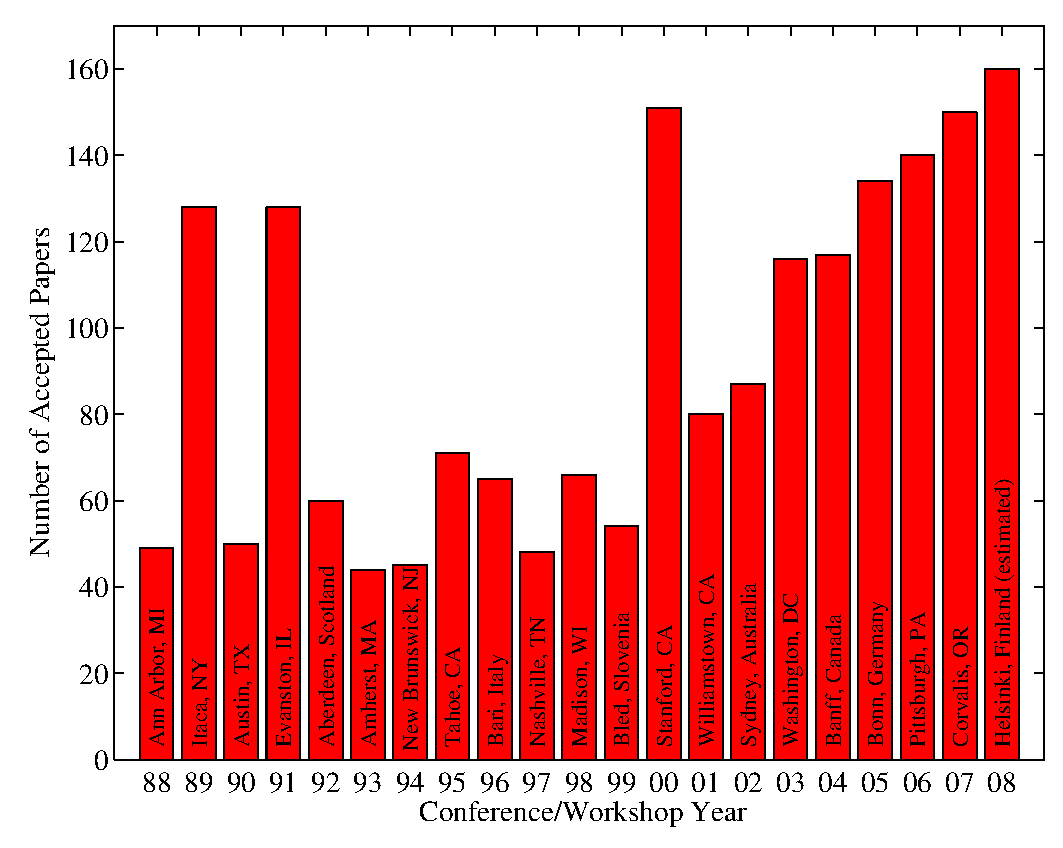
\includegraphics[width=\columnwidth]{icml_numpapers}}
\caption{Historical locations and number of accepted papers for International
Machine Learning Conferences (ICML 1993 -- ICML 2008) and International
Workshops on Machine Learning (ML 1988 -- ML 1992). At the time this figure was
produced, the number of accepted papers for ICML 2008 was unknown and instead
estimated.}
\label{icml-historical}
\end{center}
\vskip -0.2in
\end{figure}


Number figures sequentially, placing the figure number and caption
\emph{after} the graphics, with at least 0.1~inches of space before
the caption and 0.1~inches after it, as in
Figure~\ref{icml-historical}. The figure caption should be set in
9~point type and centered unless it runs two or more lines, in which
case it should be flush left. You may float figures to the top or
bottom of a column, and you may set wide figures across both columns
(use the environment \texttt{figure*} in \LaTeX). Always place
two-column figures at the top or bottom of the page.

\subsection{Algorithms}

If you are using \LaTeX, please use the ``algorithm'' and ``algorithmic''
environments to format pseudocode. These require
the corresponding stylefiles, algorithm.sty and
algorithmic.sty, which are supplied with this package.
Algorithm~\ref{alg:example} shows an example.

\begin{algorithm}[tb]
   \caption{Bubble Sort}
   \label{alg:example}
\begin{algorithmic}
   \STATE {\bfseries Input:} data $x_i$, size $m$
   \REPEAT
   \STATE Initialize $noChange = true$.
   \FOR{$i=1$ {\bfseries to} $m-1$}
   \IF{$x_i > x_{i+1}$}
   \STATE Swap $x_i$ and $x_{i+1}$
   \STATE $noChange = false$
   \ENDIF
   \ENDFOR
   \UNTIL{$noChange$ is $true$}
\end{algorithmic}
\end{algorithm}

\subsection{Tables}

You may also want to include tables that summarize material. Like
figures, these should be centered, legible, and numbered consecutively.
However, place the title \emph{above} the table with at least
0.1~inches of space before the title and the same after it, as in
Table~\ref{sample-table}. The table title should be set in 9~point
type and centered unless it runs two or more lines, in which case it
should be flush left.

% Note use of \abovespace and \belowspace to get reasonable spacing
% above and below tabular lines.

\begin{table}[t]
\caption{Classification accuracies for naive Bayes and flexible
Bayes on various data sets.}
\label{sample-table}
\vskip 0.15in
\begin{center}
\begin{small}
\begin{sc}
\begin{tabular}{lcccr}
\toprule
Data set & Naive & Flexible & Better? \\
\midrule
Breast    & 95.9$\pm$ 0.2& 96.7$\pm$ 0.2& $\surd$ \\
Cleveland & 83.3$\pm$ 0.6& 80.0$\pm$ 0.6& $\times$\\
Glass2    & 61.9$\pm$ 1.4& 83.8$\pm$ 0.7& $\surd$ \\
Credit    & 74.8$\pm$ 0.5& 78.3$\pm$ 0.6&         \\
Horse     & 73.3$\pm$ 0.9& 69.7$\pm$ 1.0& $\times$\\
Meta      & 67.1$\pm$ 0.6& 76.5$\pm$ 0.5& $\surd$ \\
Pima      & 75.1$\pm$ 0.6& 73.9$\pm$ 0.5&         \\
Vehicle   & 44.9$\pm$ 0.6& 61.5$\pm$ 0.4& $\surd$ \\
\bottomrule
\end{tabular}
\end{sc}
\end{small}
\end{center}
\vskip -0.1in
\end{table}

Tables contain textual material, whereas figures contain graphical material.
Specify the contents of each row and column in the table's topmost
row. Again, you may float tables to a column's top or bottom, and set
wide tables across both columns. Place two-column tables at the
top or bottom of the page.

% In the unusual situation where you want a paper to appear in the
% references without citing it in the main text, use \nocite
%\nocite{langley00}

\bibliography{example_paper}
\bibliographystyle{icml2021}




\end{document}

